% !TEX root = main.tex
% Tipo di documento. L'uso di twoside implica che i capitoli inizino sempre con la prima pagina a sinistra, eventualmente lasciando una pagina vuota nel capitolo precedente. Se questa cosa è fastidiosa, è possibile rimuoverlo. 
\documentclass[a4paper, twoside,openright]{report}
% \documentclass[a4paper,openright]{report}

% \usepackage{fancyhdr}
% \pagestyle{fancy}
% \fancyhf{}
% \lhead{\rightmark}
% \rhead{\textbf{\thepage}}
% % \fancyfoot{}
% \setlength{\headheight}{12.5pt}
% Rimuove il numero di pagina all'inizio dei capitoli
% \fancypagestyle{plain}{
%   \fancyfoot{}
%   \fancyhead{}
%   \renewcommand{\headrulewidth}{0pt}
% }


\usepackage{graphicx} % Required for inserting images
\setkeys{Gin}{width=0.6\columnwidth}

\usepackage[utf8]{inputenc}

\usepackage{hyperref}
\usepackage{adjustbox}

\usepackage{wrapfig}

\usepackage{enumitem}
\renewcommand{\labelitemi}{$\diamond$}
\renewcommand{\labelitemiii}{$\circ$}
\setlist[enumerate,2]{label=\roman*.}
\setlist[enumerate,3]{label=(\alph*)}

\setitemize{noitemsep}
\setenumerate{noitemsep}
\setlist{noitemsep}

\usepackage{paracol}
\usepackage{multicol}
\usepackage{booktabs}


\usepackage{geometry}

\usepackage{color}

\usepackage{listings}
% \usepackage{minted}

\usepackage{amsmath}
\usepackage{amssymb}
\usepackage{amsfonts}
\usepackage{mathtools}
\usepackage{bm}
\usepackage{nicefrac, xfrac}

\usepackage{wasysym}

% Uso dei colori
\usepackage[dvipsnames,table,xcdraw]{xcolor}
\usepackage{colortbl}
\usepackage{rotating}
\usepackage{adjustbox}

\usepackage{multirow}
\usepackage{booktabs}
\usepackage{makecell}


\usepackage{tikz}
\usetikzlibrary{automata, arrows,bending}
\usetikzlibrary{positioning}
\usetikzlibrary{shapes.geometric}
\usepackage{parskip}
\usepackage{changepage}

\usepackage{soul}
\usepackage{cancel}

% This are needed because the correct double quotes would be ``'' or ``",
% but i've always written "text"
% TODO - check whether this affects listing environment
% \usepackage [english]{babel}
% \usepackage [autostyle, english = american]{csquotes}
% \MakeOuterQuote{"}

\geometry{margin=0.6in}

\setlist[description]{itemsep=0em,topsep=0.5em,parsep=0em}
\setlist[itemize]{itemsep=0em,topsep=0pt}
\setlist[enumerate]{itemsep=0em,topsep=0pt}

\hypersetup{
    colorlinks=true,
    linkcolor=black,
    filecolor=mauve,
    urlcolor=blue,
}

\definecolor{gray}{gray}{0.3}
\definecolor{verylightgray}{gray}{0.95}
\definecolor{blue}{rgb}{0,0,1}
\definecolor{mauve}{rgb}{0.58,0,0.82}
\definecolor{darkred}{rgb}{0.3,0,0}
\definecolor{darkgreen}{rgb}{0,0.3,0}
\definecolor{darkgray}{gray}{0.15}



\newenvironment{notes}{
\par
\color{gray}
\small}

\newcommand{\note}[1]{\begin{notes}{#1}\end{notes}}
\newcommand{\nl}[0]{\parskip = \baselineskip}
\newcommand{\lst}[1]{\lstinline{#1}}
\newcommand{\ra}{\xrightarrow{\hspace*{2em}}}
\newcommand{\ns}{\setlength{\parskip}{0em}}

\newlength{\currentparindent}
\newcommand{\labelitemize}[2]{
\setlength{\currentparindent}{\parindent}
\setlength{\parindent}{0pt}

\begin{minipage}{0em} % Adjust the width as needed
    \makebox[0em][c]{\rotatebox{90}{\small #1}}
\end{minipage}
\begin{minipage}{\dimexpr\columnwidth-1cm\relax}
    #2
\end{minipage}
\setlength{\parindent}{\currentparindent}
}
\newcommand{\colfill}{\vspace{\fill}}

\newcommand{\framed}[1]{
\begin{center}
\fbox{
    \begin{minipage}{0.8\columnwidth}
        #1
    \end{minipage}
}
\end{center}}

\newcommand{\framedt}[2]{
\begin{center}
\fbox{
    \begin{minipage}{0.8\columnwidth}
        \vspace*{1em}
        \begin{center}
            \textbf{\ul{#1}}
        \end{center}
        \nl
        #2
    \end{minipage}
}
\end{center}}

\newcommand{\proscons}[4]{
    \begin{paracol}{2}
        \labelitemize{\color{darkgreen}\ul{\textit{#1}}}{
           \color{darkgreen}
           #3
        }
        \switchcolumn
        \labelitemize{\color{darkred}\ul{\textit{#2}}}{
           \color{darkred}
           #4
        }
     \end{paracol}
}

\newcommand\hcancel[2][black]{\setbox0=\hbox{$#2$}%
\rlap{\raisebox{.45\ht0}{\textcolor{#1}{\rule{\wd0}{1pt}}}}#2} 


\lstset{frame=false,
 showstringspaces=false,
 breaklines=true;
 columns=flexible,
 basicstyle={\small\ttfamily},
 keywordstyle=\color{blue},
 commentstyle=\color{darkgreen},
 stringstyle=\color{mauve}
 tabsize=3
}

\newtheorem{definition}{Definition}[chapter]
\newtheorem{theorem}{Theorem}[chapter]

\usepackage{fancyhdr}
% \usepackage{nameref,autoref}

\pagestyle{fancy}
\fancyhf{}
\fancyhead[LE,RO]{\thepage} % Page number on Outer side of header on each page
\fancyhead[LO]{\leftmark} % section title on Left side of header on Odd pages
\fancyhead[RE]{\rightmark} % subection title on Right side of header on Even pages
\fancyfoot{}
\renewcommand{\headrulewidth}{0.4pt} % Width of line under the header
% \setcounter{secnumdepth}{2} % Depth of sectioning commands to include in the table of contents

% Rimuove il numero di pagina all'inizio dei capitoli
\fancypagestyle{plain}{
  \fancyfoot{}
  \fancyhead{}
  \renewcommand{\headrulewidth}{0pt}
}

\usepackage{emptypage}



\title{Auditoría, calidad y gestión de sistemas de información - Notas}
\author{Francesco Lorenzoni}
\date{Febrero 2025}


% \makeatletter
% \renewcommand{\l@section}{\@dottedtocline{1}{1.5em}{2.6em}}
% \renewcommand{\l@subsection}{\@dottedtocline{2}{2.5em}{3.6em}}
% \renewcommand{\l@subsubsection}{\@dottedtocline{3}{3.5em}{4.5em}}
% \makeatother
% \mtcsettitle{parttoc}{Contents of this Part} % Set the title for the part TOC


\lstset{language=Java}
\begin{document}
% \doparttoc[n]

\maketitle
\tableofcontents

% \part{Introduction to ACG}
% \parttoc
\chapter{Práctica 4 y 5}

% No necesario con minted (se especifica al usar el entorno)
\lstset{language=python}

% Preface
% \note{Soy un estudiante italiano en Erasmus. Hablo español bastante bien, pero me resulta más natural escribir en inglés; sin embargo, decidí escribir en español para practicar, con la ayuda de algunos traductores cuando era necesario. Si hay algo mal escrito o poco claro, estoy a disposición para cualquier aclaración.}

\section{Ejercicios 1/2/3 - \texttt{sin\_vocales}}

\subsection{Ejercicio 1 - Función inicial}
\begin{lstlisting}[captionpos=b,caption={Función inicial}]
   def sin_vocales (s):
      """
      devuelve el argumento s sin vocales
      """
      vocales = 'aeiou'
      s_sinVocales = ' '
      for ch in s:
         pos = vocales.find(ch)
         if pos == -1: #ch no es vocal
            s_sinVocales = s_sinVocales + ch
      return s_sinVocales
\end{lstlisting}

Esta es la función inicial que se nos ha dado, y que parece funcionar, pero solo con pruebas demasiado sencillas.

\subsection{Ejercicio 2 - Prueba de la función}

Abajo en el código \ref{code:pruebas}, después de la discusión de los dos errores encontrados, hay la función	de prueba completa \lstinline{test_sin_vocales()} que comprueba la función \lstinline{sin_vocales(s)}. 


\begin{paracol}{2}
   \colfill
   El primero error en la función dada \lstinline{sin_vocales(s)} es que \ul{no se tiene cuenta de las \textbf{mayúsculas} y \textbf{minúsculas}}. Por lo tanto, la función no elimina las vocales mayúsculas. Para solucionarlo, es suficiente añadir a la lista de vocales la versión mayúscula de cada vocal.
   \colfill

   \switchcolumn

   \begin{lstlisting}
def test_sin_vocales():
   s = "el agua esta mojada"
   exp = "l g st mjd"
   assert sin_vocales(s) == exp

   ...
      
   s = "El AgUe eStA mOjAdA"
   exp = "l g St mjd"
   assert sin_vocales(s) == exp
   \end{lstlisting}
\end{paracol}

\begin{lstlisting}[captionpos=b,caption={\lstinline|sin_vocales()| con vocales mayúsculas}, label={code:sin_vocales1}]
   def sin_vocales (s:str):
      vocales = 'aeiouAEIOU'
      s_sinVocales = ''
      for ch in s:
         pos = vocales.find(ch)
         if pos == -1: #ch no es vocal
            s_sinVocales = s_sinVocales + ch
      return s_sinVocales
\end{lstlisting}

\newpage
\begin{paracol}{2}
   \colfill
   El segundo error es que la función \ul{no tiene cuenta de los \textbf{acentos}}. Por lo tanto, la función no elimina las vocales acentuadas.
   \begin{lstlisting}
   assert sin_vocales("áÉíÓú") == "" # falla
   \end{lstlisting}
   Para solucionarlo, es suficiente añadir a la lista de vocales la versión acentuada de cada vocal.

   \begin{lstlisting}
   vocales = 'aeiouAEIOUáéíóúàèìòùäëïöüâê
   îôûÁÉÍÓÚÀÈÌÒÙÄËÏÖÜÂÊÎÔÛãõÃÕ'
   \end{lstlisting}

   Esta solución no parece muy elegante, ya que la lista de vocales se vuelve muy larga. Buscando sobre el internet he visto que una solución más elegante sería usar una expresión regular para eliminar todas las vocales, acentuadas o no. Para ello, se puede usar el módulo \lstinline{re} de Python, junto con \lstinline{unicodedata}, como se muestra en el código a la derecha.
   \colfill

   \switchcolumn
   \colfill
   \begin{lstlisting}[label={code:unicodedata},captionpos=b,caption={Código para eliminar vocales y diacríticos que utiliza \lstinline{unicodedata}}]
import unicodedata
import re

def sin_vocales(s):
   # Normaliza el texto separando los caracteres básicos de sus diacríticos
   s_norm = unicodedata.normalize('NFD', s)
   # Elimina todas las vocales base y los diacríticos
   s_sin_vocales = re.sub(r'[aeiouAEIOU\u0300-\u036f]', '', s_norm)
   return s_sin_vocales
   \end{lstlisting}
   \colfill
\end{paracol}

\vspace{2em}

\begin{lstlisting}[captionpos=b,caption={Pruebas que he escrito}, label={code:pruebas}]
def test_sin_vocales():
   s = "el agua esta mojada"
   exp = "l g st mjd"
   assert sin_vocales(s) == exp
   s = "aieou"
   exp = ""
   assert sin_vocales(s) == exp
   s = "123greee"
   exp = "123gr"
   assert sin_vocales(s) == exp
   s = "El AgUe eStA mOjAdA"
   exp = "l g St mjd"
   assert sin_vocales(s) == exp
   s = "àéíóú"
   exp = ""
   assert sin_vocales(s) == exp
   s = "are you ok?"
   exp = "r y k?"
   assert sin_vocales(s) == exp
   s = ""
   exp = ""
   assert sin_vocales(s) == exp
   s = "A"
   exp = ""
   assert sin_vocales(s) == exp
   
\end{lstlisting}
\subsection{Ejercicio 3/4 - Corregir la función y añadir pruebas}

\begin{lstlisting}[captionpos=b,caption={\lstinline|sin_vocales()| corregida}, label={code:sin_vocales}]
   def sin_vocales (s:str):
      vocales = 'aeiouAEIOUáéíóúàèìòùäëïöüâêîôûÁÉÍÓÚÀÈÌÒÙÄËÏÖÜÂÊÎÔÛãõÃÕ'
      s_sinVocales = ''
      for ch in s:
         pos = vocales.find(ch)
         if pos == -1: #ch no es vocal
            s_sinVocales = s_sinVocales + ch
      return s_sinVocales
\end{lstlisting}

Para evitar el uso del paquete adicional \lstinline{unicodedata}, he preferido utilizar simplemente listas de vocales que incluyen también las vocales acentuadas.

He añadido al fichero \texttt{.py} la función que nos ha dado en el ejercicio, per controllare che anche quei test passassero.

\newpage
\section{Ejercicio 5 - \texttt{cantidad\_numeros}}
\begin{lstlisting}[captionpos=b,caption={Solución sencilla}]
def cantidad_numeros_sencilla(s: str):
   """
   Esta función recibe una cadena de texto y devuelve la cantidad de números que contiene.
   N.B. números, no digitos!
   """
   return len(re.findall(r'\d+', s))
\end{lstlisting}

Esta primera solución funciona y es concisa, pero no tiene en cuenta los números decimales (como $12.34$) y las notaciones científicas (como $12\cdot 10^6$ o $10^{-2}$). 
Para solucionarlo, es necesario modificar la expresión regular para que también considere estos casos.

\begin{lstlisting}[captionpos=b,caption={Solución que incluye números decimales y notaciones científicas}]
      
def cantidad_numeros(s: str):
   """
   Esta función recibe una cadena de texto y devuelve la cantidad de números que contiene.
   
   Números decimales (como 12.34) y notaciones científicas (como 12*10^6 o 10^(-2)) son considerados números.
   """
   # Identificar números decimales (como 12.34)
   decimal_pattern = r'-?\d+\.\d+'
   decimal_matches = re.findall(decimal_pattern, s)
   
   # Eliminar los números decimales ya encontrados para evitar contar dos veces
   for match in decimal_matches:
       s = s.replace(match, ' ', 1)
   
   # Identificar notaciones científicas (como 12*10^6 o 10^(-2))
   scientific_pattern = r'\d+\*10\^\(?\-?\d+\)?'
   scientific_matches = re.findall(scientific_pattern, s)
   
   # Eliminar las notaciones científicas de la cadena
   for match in scientific_matches:
       s = s.replace(match, ' ', 1)
   
   # Encontrar los números restantes (enteros)
   # Modificamos el patrón para capturar secuencias de dígitos en cualquier contexto
   remaining_pattern = r'\d+'
   remaining_matches = re.findall(remaining_pattern, s)
   
   # Contar el total de números encontrados
   return len(decimal_matches) + len(scientific_matches) + len(remaining_matches)
\end{lstlisting}

\newpage
\begin{paracol}{2}
   
   \begin{lstlisting}[captionpos=b,caption={Mis pruebas para \lstinline|cantidad_numeros()|}, label={code:cantidad_numeros}]
def test_cantidad_numeros():
   s = "12 356 53333"
   assert cantidad_numeros(s) == 3
   s = "asfa432asf23"
   assert cantidad_numeros(s) == 2
   s = ""
   assert cantidad_numeros(s) == 0
   s = "1"
   assert cantidad_numeros(s) == 1
   s = "fwgds"
   assert cantidad_numeros(s) == 0
   s = "1 fhsdSGG 4"
   assert cantidad_numeros(s) == 2
   s = "-12 + 34 -12-133 "
   assert cantidad_numeros(s) == 4
   s = "12.34 56.78"
   assert cantidad_numeros(s) == 2
   s = "12*10^6"
   assert cantidad_numeros(s) == 1
   s = "23*10^(-2)"
   assert cantidad_numeros(s) == 1
   s = "23*10^(64) + 12.34"
   assert cantidad_numeros(s) == 2
   s = "asgre23*10^(-2)asfg10^2"
   assert cantidad_numeros(s) == 2
   s = "asgre23*10^(-2)asfg10^2agr12.34"
   assert cantidad_numeros(s) == 3
   \end{lstlisting}

   \switchcolumn

   \begin{lstlisting}[captionpos=b,caption={Pruebas ordenadas como estan en el documiento}, label={code:cantidad_numeros2}]
def test_cantidad_numeros_doc():
   # Varios números en la cadena
   s = "un 1, un 201 y 2 unos"   
   assert cantidad_numeros(s) == 3
   # Sin números en la cadena
   s = "sin numeros"   
   assert cantidad_numeros(s) == 0
   # Un solo número en la cadena
   s = "2345543"    
   assert cantidad_numeros(s) == 1
   # Diferentes longitudes de números
   s = "1 22 333 4444 55555"    
   assert cantidad_numeros(s) == 5
   # Números separados por espacios
   s = "123 456 789"    
   assert cantidad_numeros(s) == 3
   # Números separados por comas
   s = "12,34,56,78"    
   assert cantidad_numeros(s) == 4
   # Números rodeados de texto
   s = "numero123numero456numero"   
   assert cantidad_numeros(s) == 2
   # Una cadena continua de números
   s = "123456789"   
   assert cantidad_numeros(s) == 1
   # Números al inicio y al final
   s = "1 starting and ending 2"    
   assert cantidad_numeros(s) == 2
   # Número al final 
   s = "ending with number 5"   
   assert cantidad_numeros(s) == 1
   # Números en una cadena simple
   s = "3 6 9"   
   assert cantidad_numeros(s) == 3
   # Sin números en la cadena
   s = "sinnumeros"    
   assert cantidad_numeros(s) == 0
   # Números mezclados con texto
   s = "123unnumero456"   
   assert cantidad_numeros(s) == 2
   # Números negativos
   s = "-5 10 -15"  
   assert cantidad_numeros(s) == 3
   \end{lstlisting}
\end{paracol}

\newpage
\section{Ejercicio 6 - \texttt{sin\_vocales} con prueba parametrizada}

\begin{lstlisting}
@pytest.mark.parametrize ("entrada , salida_esperada " ,[
   ("El agua esta mojada", "l g st mjd"),
   ("mojada bañando en el agua", "mjd bñnd n l g"),
   ("ahora termina bien", "hr trmn bn"),
   ("", ""),
   ("a", ""),
   ("m", "m"),
   ("unstringsinespacios", "nstrngsnspcs"),
   ("MAYUSculas FUNCIOnaN", "MYScls FNCnN"),
   ("krt yhgf dwpq", "krt yhgf dwpq"),
   ("aeoiuuuoiea", ""),
   ("disco de los 80", "dsc d ls 80"),
   ("signos como ? y ! y ¡", "sgns cm ? y ! y ¡"),
   ("ábc élla ó", "bc ll "),
   ("Óm tambien mayÚsculÁs", "m tmbn myscls")
   ])

def test_sin_vocales_parametrizado(entrada, salida_esperada):
   """
   testea la función sin_vocales
   """
   assert sin_vocales (entrada) == salida_esperada
\end{lstlisting}

Esta es una forma alternativa de escribir los test, que permite de parametrizar la función driver de test.

En comparación con el test set anterior del pdf, hemos añadido pruebas que incluyen vocales con acento. La función \lstinline|sin_vocales| no va a cambiar porque ya había tenido en cuenta los acentos en el ejercicio anterior.




\chapter{Estrategias de Testing}
\label{chap:estrategias-de-testing}

El proceso de testng dentro de un proyecto de software es una actvidad que tene como objetivo \ul{verificar} y \ul{validar} que el software cumple con los requisitos especificados.

El proceso de testing conlleva:
\begin{itemize}
	\item planificación,
	\item diseño,
	\item ejecución de pruebas y
	\item evaluación
\end{itemize}
La gestión de calidad debe garan2zar que el proceso de
testing se lleve a cabo de manera eficiente y eficaz.

\section{Tipos de Testing}
\begin{itemize}
	\item Testeo \textbf{unitario}\\
   Testeo de unidades de software individuales
	\item Testeo de \textbf{integración}\\
   Testeo de los interfaces de y la interacción entre las unidades previamente testeadas
	\item Testeo de \textbf{sistema}\\
   Testeo del sistema entero
	\item Testeo de \textbf{aceptación}\\
   Testeo del sistema y los criterios de aceptación previamente establecidos con el cliente
\end{itemize}

\subsection{Testeo Unitario}
Las \textbf{unidades} son Clases/Métodos (en OO), Procedimientos, Módulos o Componentes. Como se definen las unidades depende del diseño, de la criticidad del software (más crítico implica unidades más pequeñas), de la empresa (estrategia), o del tiempo disponible.


Una \textbf{prueba unitaria} (\texttt{unit test}) es una pieza de código escrita por un desarrollador que pone a prueba un pequeño y específico trozo de código.
Es una manera relativamente barata para mejorar la calidad del código producido, pero \textit{NO} es para usuarios, gerentes, jefes de proyectos: està hech para los programadores.
El programador examina o ejecuta una pequeña
parte de su código, para testear:
\ul{la funcionalidad que él o ella piensa que tiene que tener}

\begin{figure}[htbp]
   \centering
   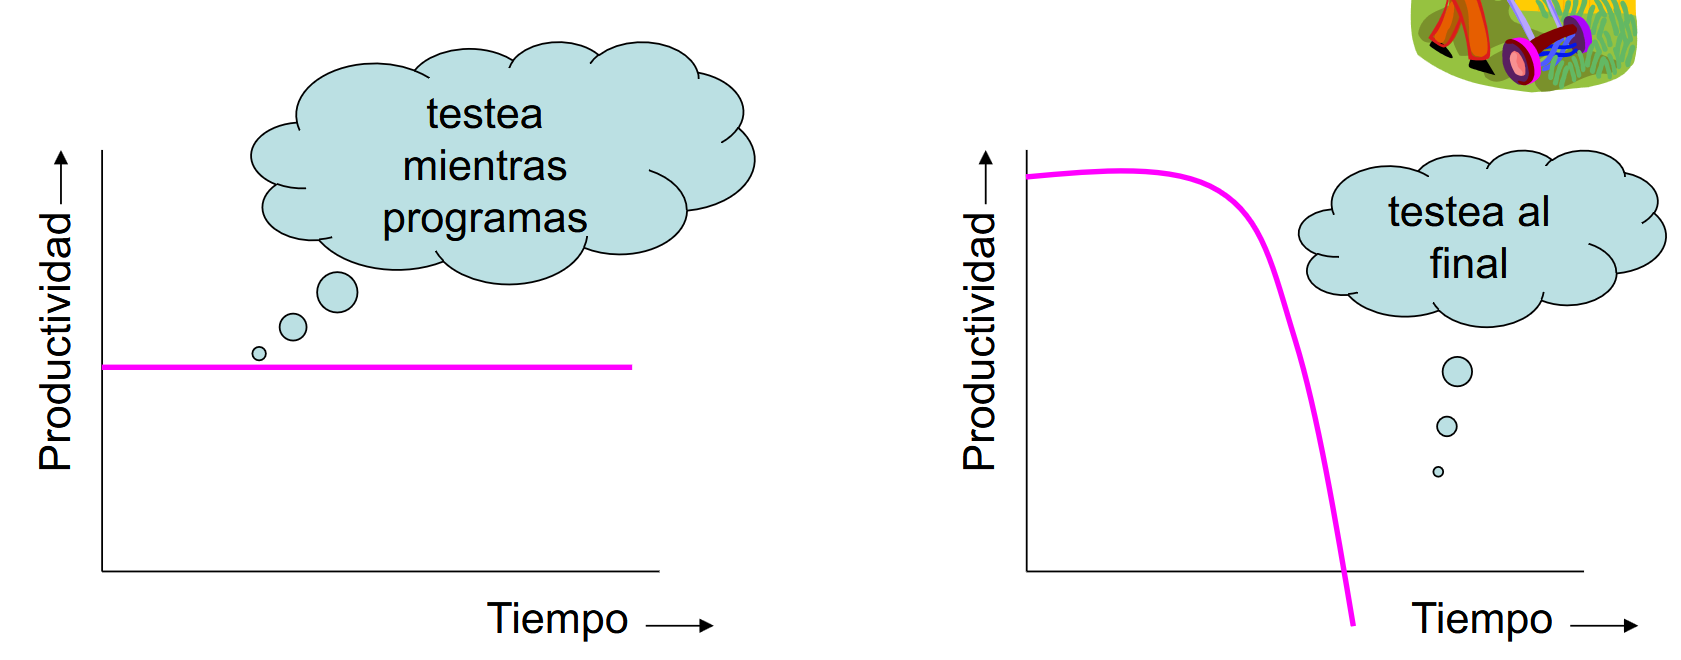
\includegraphics{images/03/unitPostpone.png}
   \caption{Posponer el testeo unitario cuesta mucho tiempo}
   \label{fig:03/unitPostpone}
\end{figure}

\coolquote{
   No es mi trabajo hacer testeo, tenemos un departamento de calidad
}{Bad programmer}

Entonces ¿cuál es el trabajo de un programador? El trabajo de cada programador es \ul{producir código que
funciona y que no contenga ``muchos'' errores}

\subsubsection{JUnit}

\begin{paracol}{2}
	
	\colfill
	JUnit es un framework de testing para Java. JUnit es una herramienta que ayuda a los programadores a escribir pruebas unitarias en Java. JUnit ha sido importante en el desarrollo de la metodología de programación extrema (XP).
	\lstinline|@Test| son los métodos de prueba.
	\begin{itemize}
		\item \lstinline|@BeforeEach| se invoca antes de la ejecución de cada test
		\item \lstinline|@AfterEach| se invoca después de la ejecución de cada test
		\item \lstinline|@BeforeAll| se invoca antes de la ejecución de todos los tests
		\item \lstinline|@AfterAll| se invoca después de la ejecución de todos los tests
	\end{itemize}
	
	\colfill
	\switchcolumn

	\begin{lstlisting}
public class TestDB {
	static private Connection dbConn;
	static private Account acc;
	@BeforeAll
	public static void setUpBeforeAll(){
		dbConn = new Connection("Oracle",15,fred, "f");
		dbConn.connect();
	}
	@AfterAll
	public static void tearDownAfterAll(){
		dbConn.disconnect();
		dbConn = null;
		}
	@BeforeEach
	protected void setUp(){
		acc = new Account();
		}
	@AfterEach
	protected void tearDown(){
		acc = null;
	}
	
	public void testAccountAccess(){
	.../Uses dbConn and acc
	}
	public void testEmployeeAccess(){
		.../Uses dbConn and acc
		}
\end{lstlisting}			
\end{paracol}

\begin{paracol}{2}
	
	\colfill
	En el ejemplo anterior, se muestra un test de una clase \texttt{Account} que tiene una conexión a una base de datos. Se puede ver que se crea una conexión a la base de datos en el método \texttt{setUpBeforeAll} y se cierra en el método \texttt{tearDownAfterAll}. Además, se crea una instancia de la clase \texttt{Account} en el método \texttt{setUp} y se destruye en el método \texttt{tearDown}.
	\colfill
	
	\switchcolumn
	Los metodos son ejecutados en el siguiente orden:
	\ns
	\begin{itemize}
		\item \lstinline|setUpBeforeAll|
		\item \lstinline|setUp|
		\item \lstinline|testAccountAccess|
		\item \lstinline|tearDown|
		\item \lstinline|setUp|
		\item \lstinline|testEmployeeAccess|
		\item \lstinline|tearDown|
		\item \lstinline|tearDownAfterAll|
	\end{itemize}
\end{paracol}

% TODO ejemplo factorial

\subsection{Testeo de Integración}

\begin{definition}
	[Testeo de Integración]
	El testing de las interfaces y la
	interacción entre las unidades previamente testeadas
	mientras que se ensambla el sistema entero
\end{definition}

\begin{itemize}
	\item ¿Qué componentes son el foco del testeo de integración?
	\item ¿En qué orden vamos a testear las interfaces?
	\item ¿Qué técnicas utilizamos para testear las interfaces?
\end{itemize}

Hay tres estrategias:
\begin{enumerate}
	\item \textbf{Big Bang} (todos los componentes a la vez)
	\item \textbf{Bottom-up} (de abajo hacia arriba)
	\item \textbf{Top-down} (de arriba hacia abajo)
\end{enumerate}

\begin{figure}[htbp]
	\centering
	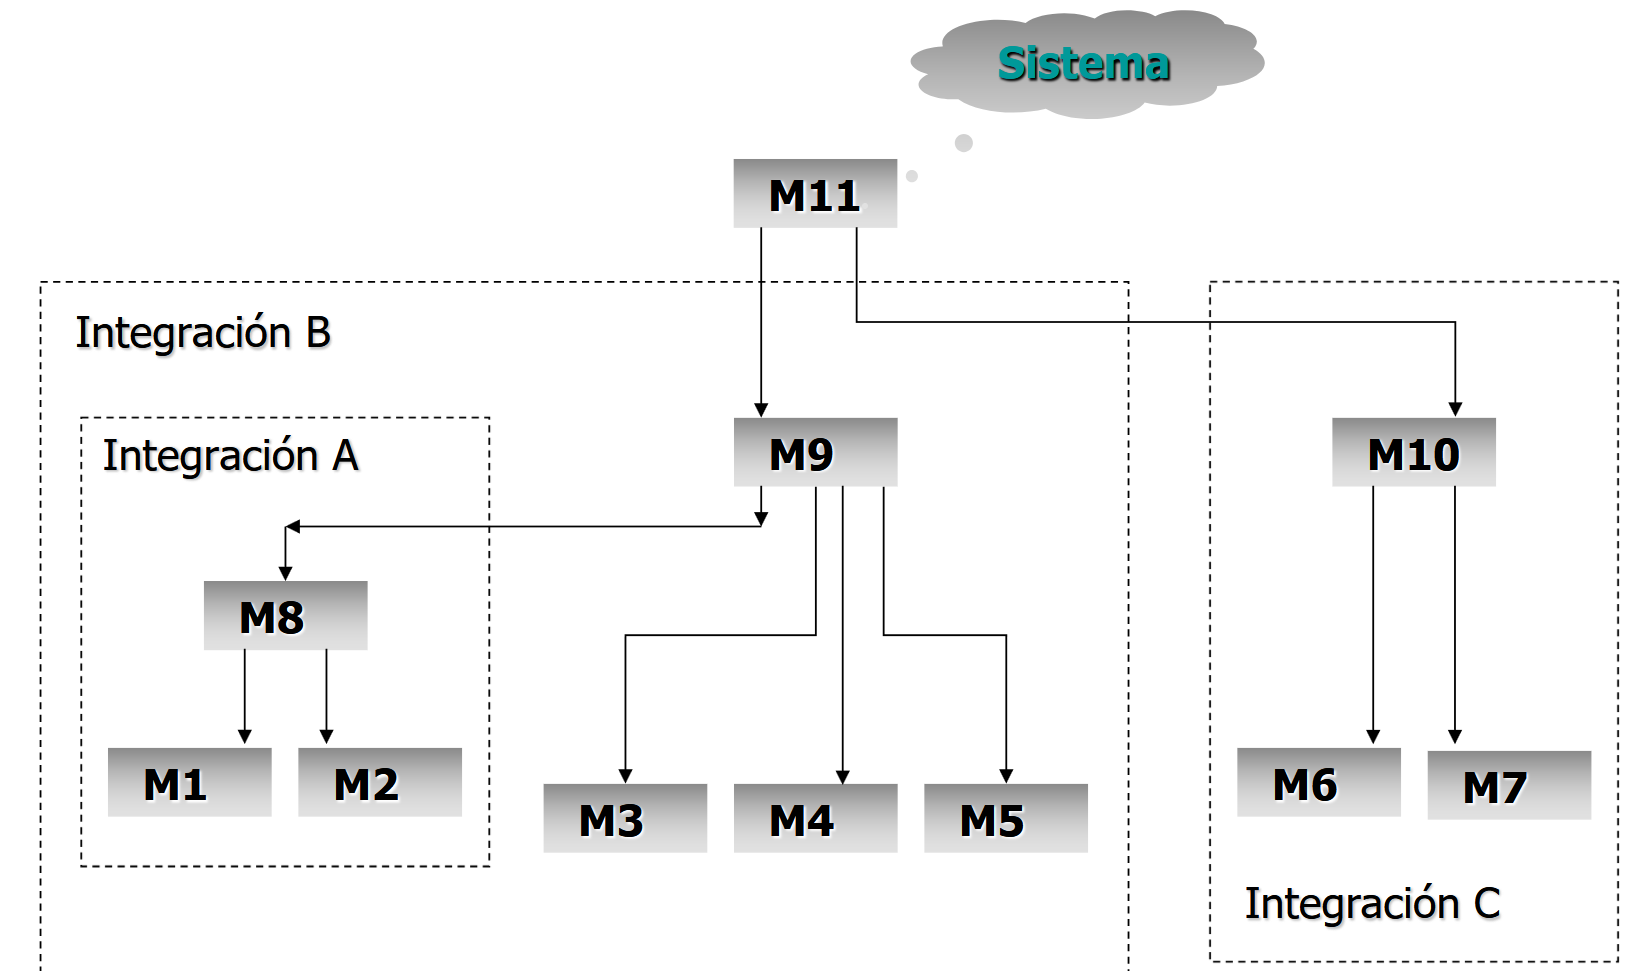
\includegraphics{images/03/bottomup.png}
	\caption{Arbol de dependencia y Bottom-up testing}
	\label{fig:03/bottomup}
\end{figure}

Para hacer el testing \textit{bottom-up} necesitamos \textbf{drivers}.
Un driver es un programa que invoca un componente bajo testeo, por ejemplo, para simular un componente de un nivel superior cuyo código todavía no está disponible (está todavía en desarrollo).

\begin{figure}[htbp]
	\centering
	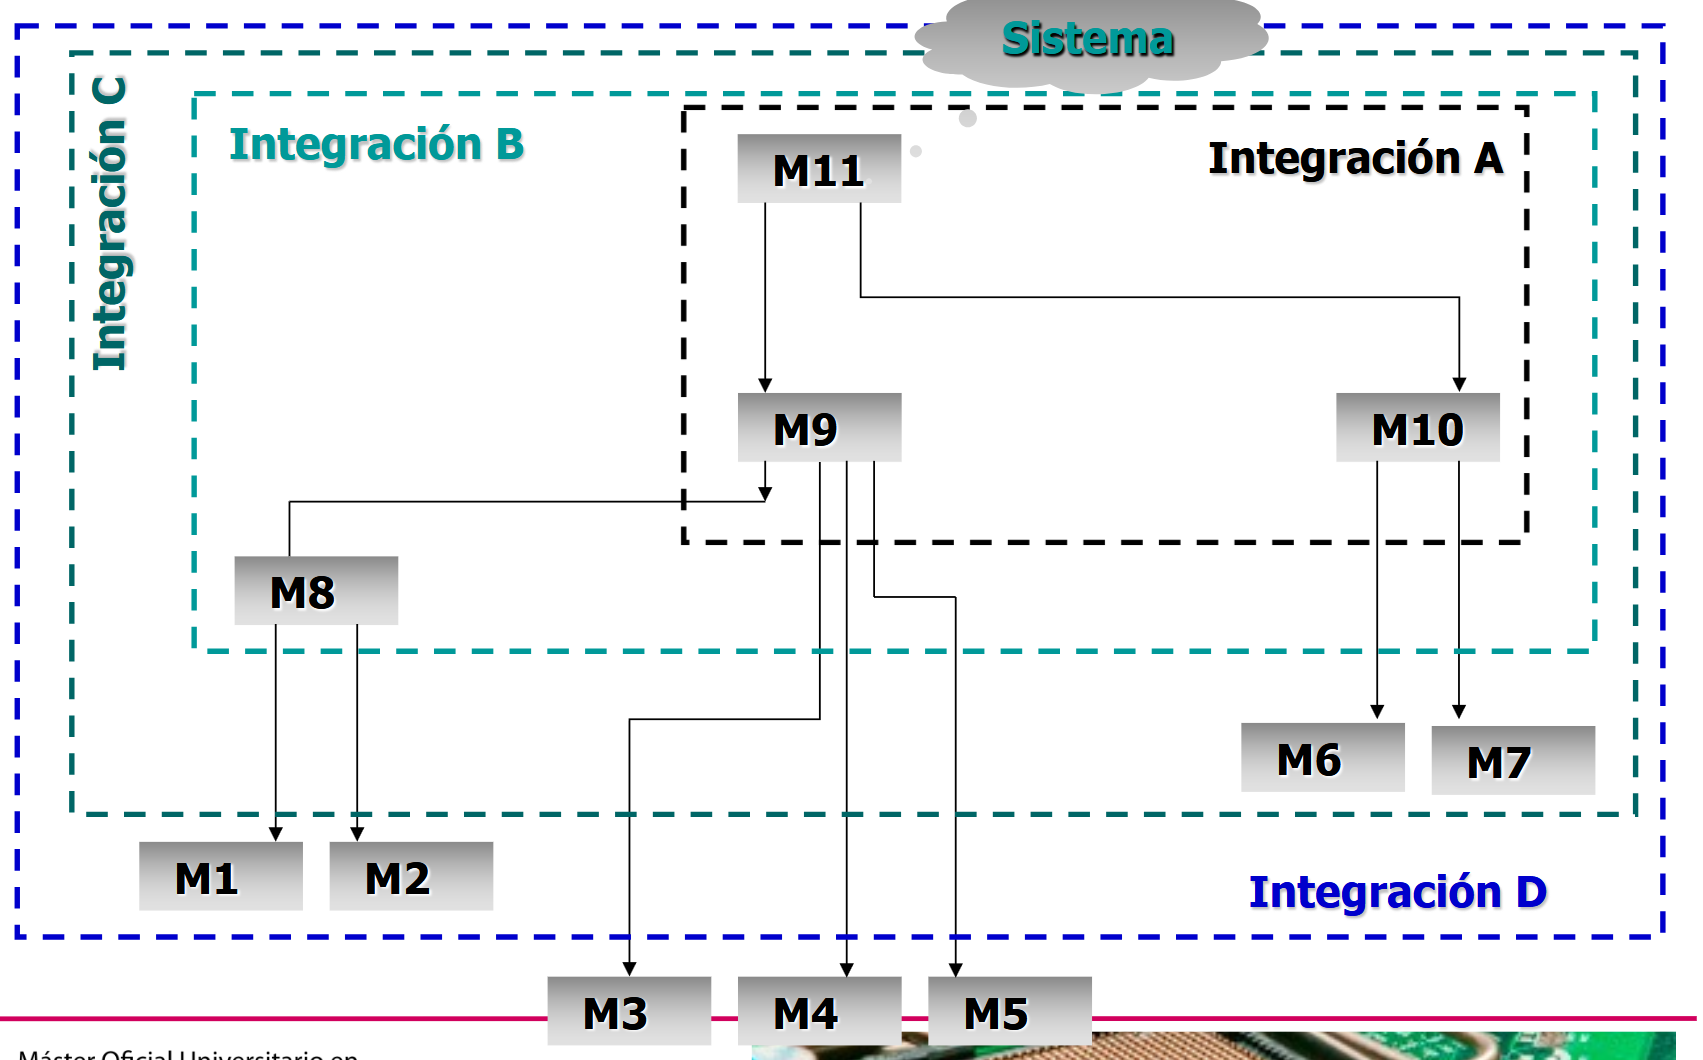
\includegraphics{images/03/topdown.png}
	\caption{Top-down testing}
	\label{fig:03/topdown}
\end{figure}

Para hacer el testeo de integración de manera \textit{top-down}, se
necesita dobles, que simulan componentes de un nivel inferior (``Stub'', ``dummy'', ``fake'', ``mock'').
\ns

El \textit{Big Bang} testing se utiliza solo para sistemas pequeños, ya que es muy difícil de manejar en sistemas grandes.


\subsubsection{Mockito}
Mockito es un framework de testing para Java que permite crear objetos simulados (mocks) de clases y interfaces. Mockito se utiliza para simular objetos que son necesarios para realizar pruebas unitarias. Se puede integrar con JUnit para realizar pruebas unitarias en Java. 
En las slides se muestran ejemplos de cómo utilizar Mockito.

Mockito es muy comodo para implementar el testeo de integración de manera \textit{top-down}.
% TODO Parte 2 y 3	

\section{Testeo de Sistema}
Se verifica que se cumple los requisitos especificados, es decir, que el sistema realiza correctamente todas las funcionesque se han detallado en las especificaciones dadas por el usuario del sistema.

Es necesario automatizar las prubas, y por esto se utilizan herramientas como \textit{Selenium}, que permite automatizar pruebas en navegadores web: en este caso, hablamos de pruebas de \textbf{funcionalidad}.

Para testar el \textbf{rendimiento} (tiempo de respuesta, carga, memoria.) se utilizan herramientas como \textit{JMeter} o \textit{NeoLoader}.

Otros aspectos importantes que el testeo debe cubrir son \textbf{Seguridad} y \textbf{Usabilidad}.

\section{Testeo de aceptación}
Esto testeo es dirigido a los criterios de aceptación
previamente establecidos con el cliente. Se puede hacer de manera manual o automatizada.

\subsection{Regresión}
Testeo que se necesita hacer después de cambios en el
software para asegurar que no se ha introducido defectos.

\ul{El testeo de \textbf{regresión} se tiene que automatizar} por el simple hecho de que el testeo de regresión manual \textit{NO SE HACE}.

\section{Gestión de Defectos, métricas y mas}

{El proceso de clasificación de defectos incluye tres fases:\ns
\begin{enumerate}
	\item Detección de defectos
	\item Investigación de defectos
	\item Resolución de defectos
\end{enumerate}}

\note{
\begin{itemize}
	\item \textbf{Actividad} (que estábamos haciendo cuando encontramos el fallo)
	\item \textbf{Fase del proyecto} (en que estábamos cuando encontramos el fallo)
	\item \textbf{Repetitividad} (¿se puede repetir el error?)
	\item \textbf{Síntoma} (fallo del sistema, mensaje de error, entrada no aceptado, resultado
incorrecto, etc.)
	\item \textbf{Causa} (nuestro producto, componente externo, usuario, etc.)
	\item \textbf{Origen} (especificación de requisitos, diseño, programación, etc.)
	\item \textbf{Impacto} (misión: crítico, medio, …; en la planificación; para el cliente, etc.)
\end{itemize}
}

\subsection{Métricas}


 Las métricas son observaciones cuantitativas para:
\begin{itemize}
	\item Informar sobre el \textbf{progreso del proyecto} de testeo
\note{\begin{itemize}
	\item ¿Qué tareas han terminado en tiempo?
	\item ¿Qué tareas han terminado antes?
	\item ¿Qué tareas han tenido retraso?
	\item ¿Cómo vamos siguiendo la planificación?
	\item Si no vamos bien, ¿cuáles son las razones?
	\item ¿Qué productividad ha tenido persona/equipo X?
\end{itemize}}
	\item Informar sobre la \textbf{calidad del software}
	\note{\begin{itemize}
		\item ¿Podemos parar el testeo?
	\item ¿Podemos entregar producto?
	\item ¿Hemos resueltos todos los defectos?
	\item ¿Cómo estamos gesHonando los defectos?
	\item ¿Cuántos defectos hemos encontrado por: subsistema,
	origen, causa, severidad, etc\dots?
	\end{itemize}}
	\item Informar sobre la \textbf{calidad del testeo}
	\note{\begin{itemize}
		\item ¿Estamos haciendo los tests necesarios?
		\item ¿Están siendo efectivos los tests?
		\item ¿Estamos utilizando los casos de prueba adecuados?
		\item ¿Necesitamos tener en cuenta diferentes casos de prueba?
	\end{itemize}}
\end{itemize}

La cobertura del testeo es una métrica importante para evaluar la calidad del testeo. La cobertura del testeo es la medida de la cantidad de código que ha sido ejecutado por los tests, especialmente en lo que se refiere a instrucciones, decisiones y condiciones (múltiples).\\
Pero puede referirse también a la cobertura de los requisitos, de los casos de uso, de los casos de prueba, etc.

\begin{lstlisting}[caption={Con 1 test donde \lstinline|x==y| se cubre todo el codigo, pero no todas las decisiones. En efecto, el defecto ocurre cuando \lstinline|x!=y|}]
	int foo_3 ( ) {
		int* p = NULL;
		int x;
		if (x==y) {
			p = &x;
		}
		*p = 123;
	}
\end{lstlisting}

\subsection{Mutación}

La mutación es una técnica de testing que consiste en introducir errores en el código fuente para ver si los tests son capaces de detectarlos. Se puede utilizar para evaluar la calidad de los tests.

\subsection{Organización del testing}
Se puede dedicar un equipo de testo integrado, con un jefe, o se puede haber que desarrolladores y testeadores son las mismas personas y no hay testeadores a tiempo completo.
La ventaja de tener un equipo de testeo es que se puede tener una visión más objetiva del software, ya que los testeadores no han desarrollado el software; al contrario, si los desarrolladores hacen el testeo, no tienen que comunicar con los testeadores, y conocen el software.

Otra tecnica de organización es \textit{Outsourcing}, que consiste en contratar una empresa externa para hacer el testeo. La ventaja es que se puede tener una visión más objetiva del software, y se puede tener acceso a expertos en testeo. La desventaja es que se puede tener problemas de comunicación, y que se puede tener problemas de confidencialidad.


\chapter{Diseño de casos de prueba}
\begin{tikzpicture}[node distance=1.5cm]
   \node (model) [rectangle, draw] {Make a model};
   \node (coverage) [rectangle, draw, below of=model] {Pick a coverage criterion};
   \node (testcases) [rectangle, draw, below of=coverage] {Design test cases};

   \draw [->] (model) -- (coverage);
   \draw [->] (coverage) -- (testcases);
\end{tikzpicture}

\section{Modelos}
\note{Recuerda que el SUT (System under test) es el sistema bajo prueba.}

\subsection{Clases de equivalencia}

Se modela el input domain, y para ello se utilizan clases de equivalencia.
Es importante notar que las clases de equivalencia son una asunción, y no una verdad absoluta, pueden ser erróneas.
\begin{paracol}{2}
   
   Sea $R$ una relación de equivalencia sobre un
   conjunto $A$. Para cada $a \in A$, llamaremos
   clase de equivalencia de $a$, al conjunto
   formado por todos los elementos de $A$ que
   estén relacionados con él a través de $R$.
   
   \switchcolumn

   \begin{figure}[htbp]
      \centering
      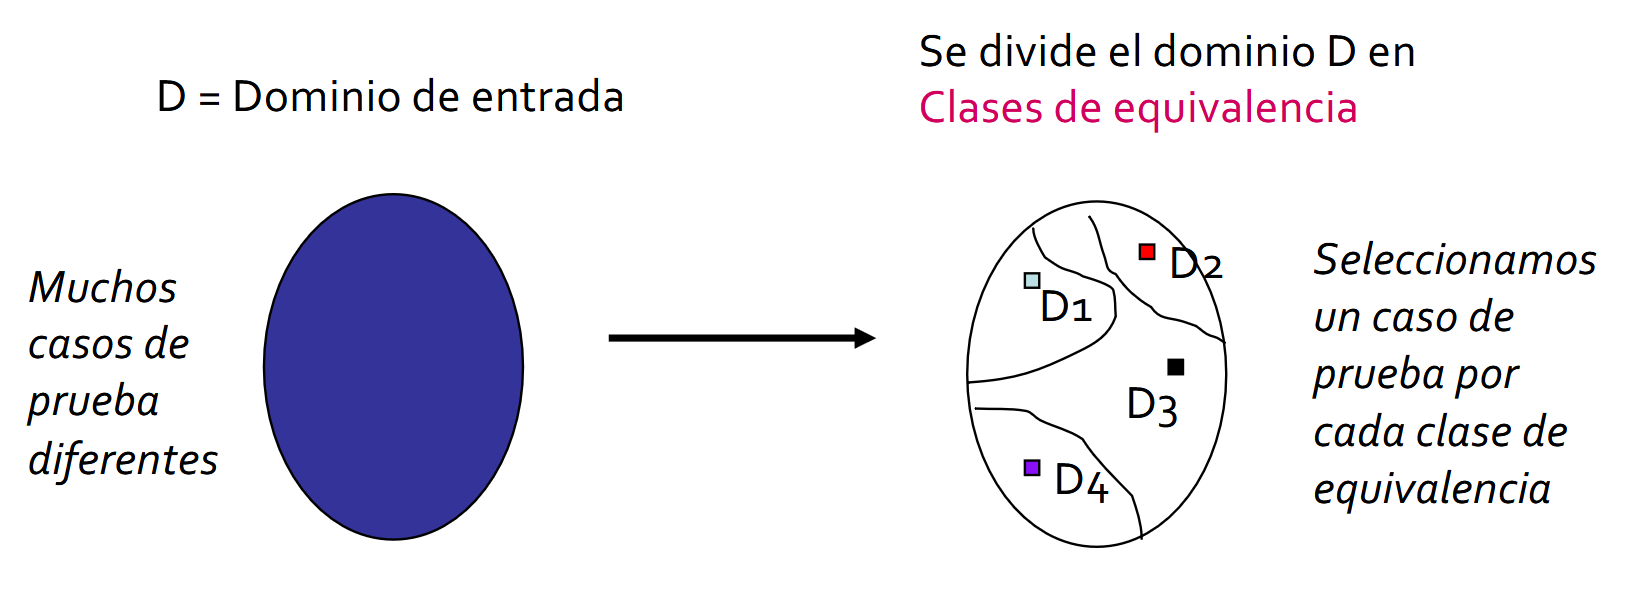
\includegraphics{images/05/claseequivalencia.png}
      \caption{Dividir el dominio}
      \label{fig:05/claseequivalencia}
   \end{figure}
\end{paracol}

Este modelo permite identificar conjuntos de pruebas de tamaño manejable seleccionando unos pocos casos de prueba para cada clase de equivalencia.
Permite también medir la efectividad de la prueba en términos de cobertura relacionada con el modelo de partición creado.
Además, el proceso de partición obliga al tester a pensar sistemáticamente sobre lo que importa

\begin{figure}[htbp]
   \centering
   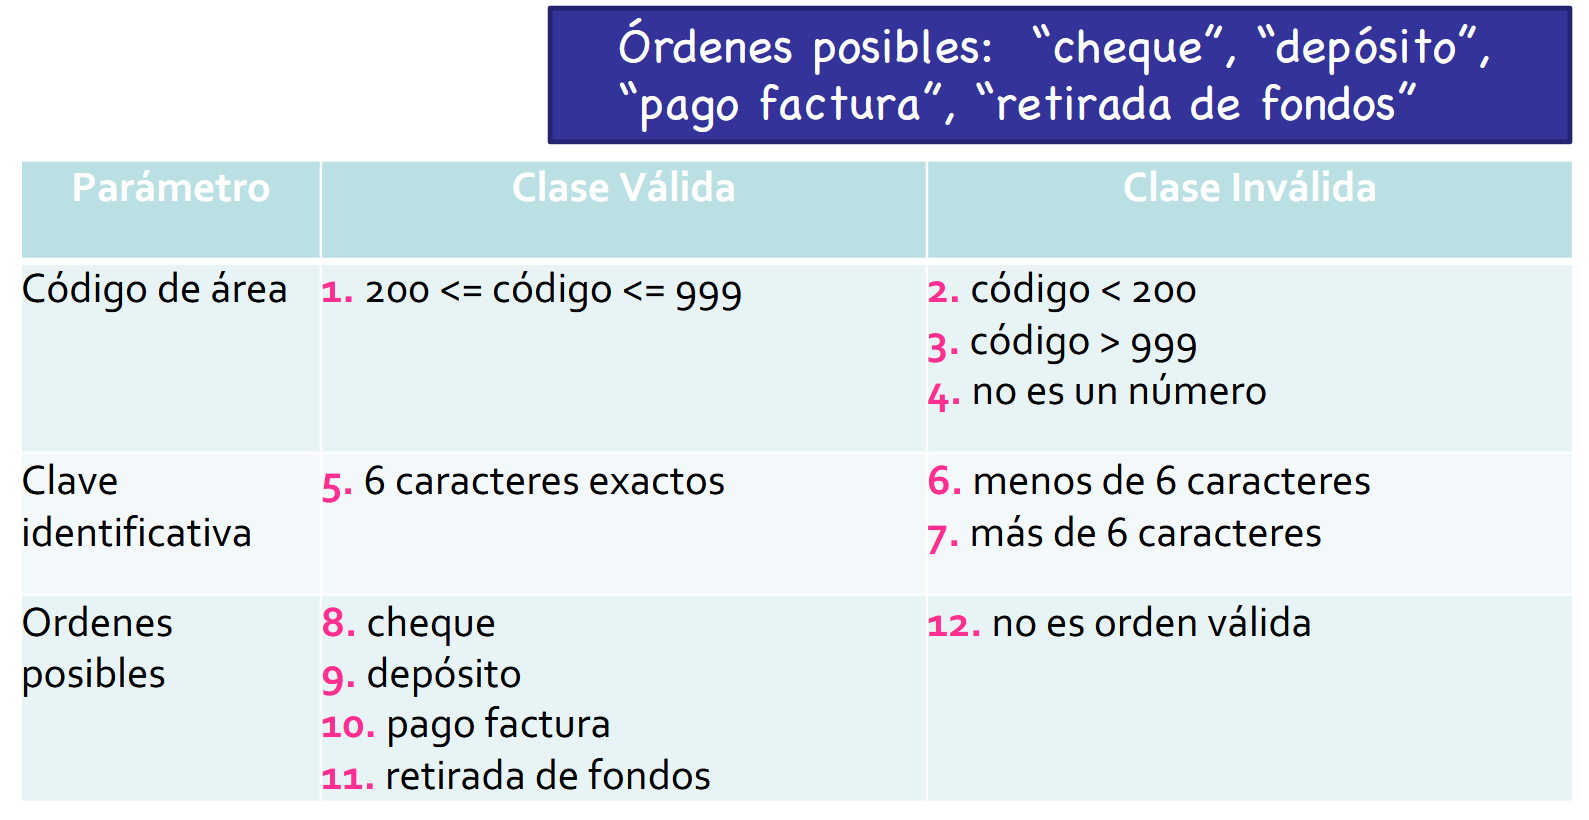
\includegraphics{images/05/claseBanca.png}
   \caption{Ejemplo de una aplicación bancaria}
   {Los datos de entrada son:\ns
   \begin{itemize}
   	\item Código de area: número de tres dígitos que no empieza ni por 0 ni por 1
	\item Clave identificativa de la operación: 6 caracteres alfanuméricos
	\item Órdenes posibles: ``cheque'', ``depósito'', ``pago factura'' , ``retirada de fondos'' 
   \end{itemize}}
   \label{fig:05/claseBanca}
\end{figure}

Es importante enumerar las clases de equivalencia, y no mezclarlas sobre todo.
Cuando se va a escribir las pruebas, cada prueba tiene que ser relacionada con una o más clases de equivalencia, y tenemos que indicar a cuales.

\begin{table}[htbp]
   \centering
   \begin{tabular}{|c|c|c|}
   \hline
       Parámetro & Clase Válida & Clase Inválida \\ \hline
       Capital & $c > min$ & $c \leq min$ \\ \hline
       Ingreso & $i \geq 0$ & $i < 0$ \\ \hline
       Deuda & $d \geq 0$ & $d < 0$ \\ \hline
       Impagados & $T \vee F$ & \\ \hline
       \multirow{4}{*}{Impagados $\wedge$ cond} & 1) $T \wedge (i - d) < c/3$  & ~ \\
       & 2) $F \wedge (i - d) \geq c/3$ & \\
       & 3) $T \wedge (i - d) \geq c/3$ & \\
       & 4) $F \wedge (i - d) < c/3$ & \\ \hline
   \end{tabular}
   \caption{Ejemplo de clases de equivalencia para una aplicación bancaria}
   \note{
   \begin{itemize}
   	\item si el cliente está en una lista de impagados y el sueldo bruto menos la deuda
   	      es inferior al capital solicitado dividido entre 3, la solicitud pasa a No
   	      Concedida.
   	\item si el cliente no está en ninguna lista, y el sueldo bruto menos la deuda es
   	      mayor o igual al capital solicitado dividido entre 3, se clasifica como Pre-
   	      concedida.
   	\item en cualquier otro caso pasa a En estudio
   \end{itemize}
   }
   \label{tab:05/claseEquivalencia}
\end{table}

\section{Tablas de decisión}

Se puede utilizar para programas que toman decisiones basadas en condiciones lógicas sobre combinaciones de entradas, parámetros y/o variables, eligiendo diferentes acciones o respuestas.
\note{\begin{itemize}
	\item La acción o respuesta que se toma no depende del orden en que
se evalúa los valores de los parámetros y variables.
	\item La acción o respuesta que se toma no depende de entradas o
salidas anteriores
\end{itemize}}

\begin{paracol}{2}
   \begin{itemize}
   	\item Cada condición corresponde a una variable, relación o predicado
	\item Valores posibles para las ``Condition Entries''
 \begin{itemize}
 	\item Booleano (\lstinline|True / False|) - Tabla de decisión de entrada limitada
	\item Valores - Tabla de decisión de entrada extendida
	\item Valor ``No Importa'' (Don't care value)

 \end{itemize}
\item Cada acción es una operación que hay que ejecutar

   \end{itemize}
\switchcolumn
\begin{figure}[htbp]
   \centering
   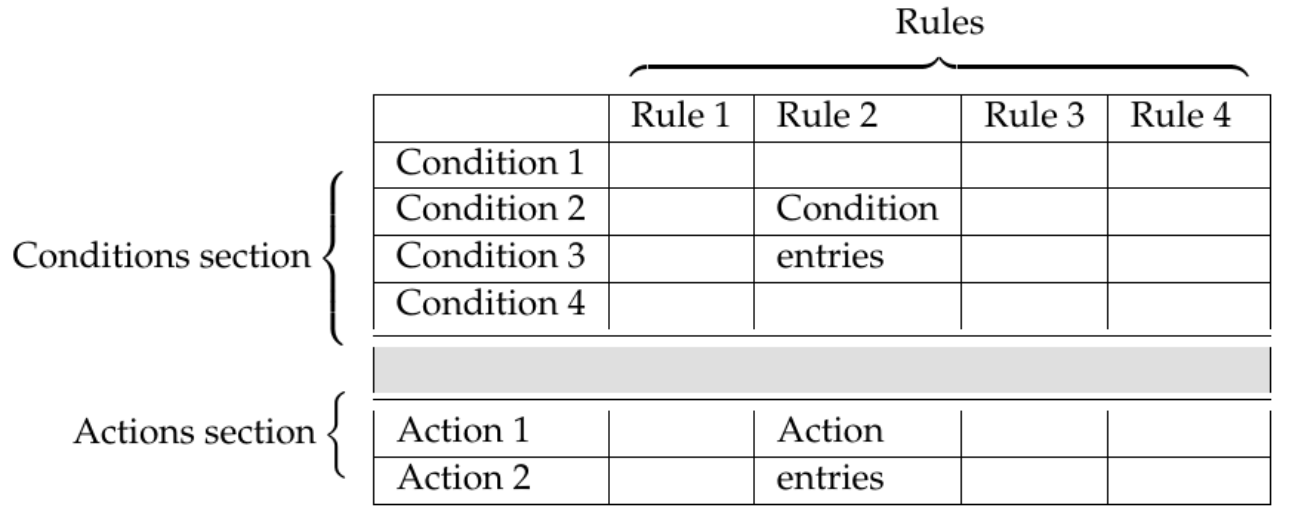
\includegraphics{images/05/tabladecision.png}
   \caption{Tabla decision }
   \label{fig:05/tabladecision}
\end{figure}
\end{paracol}

\begin{figure}[htbp]
   \centering
   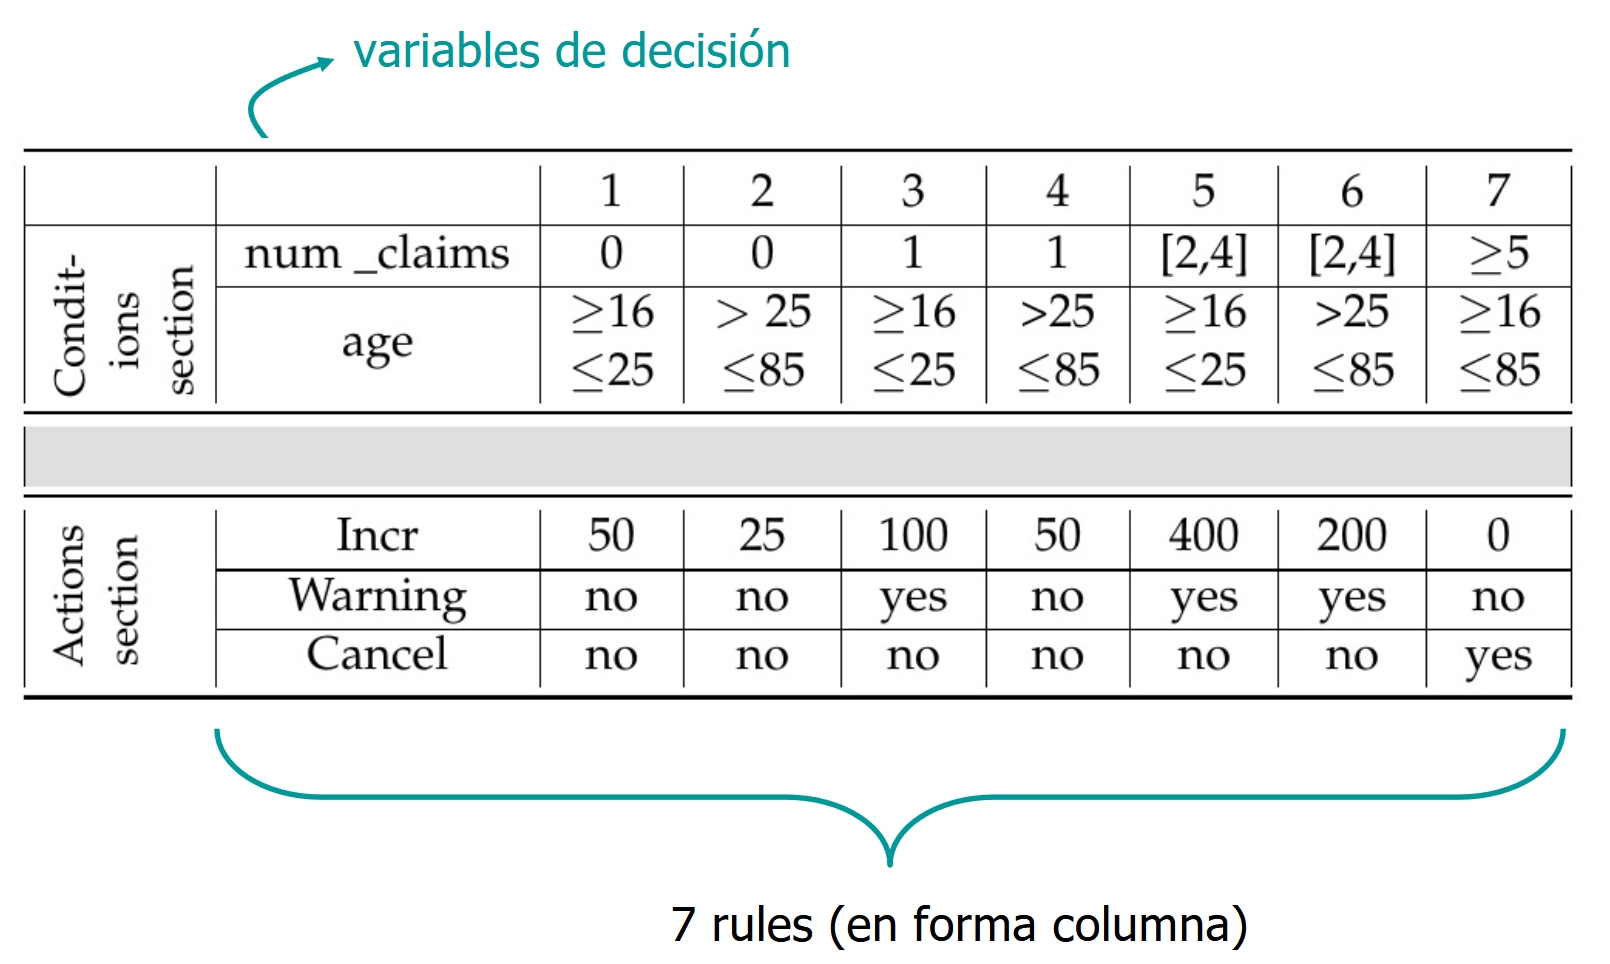
\includegraphics{images/05/tablaForma1.png}
   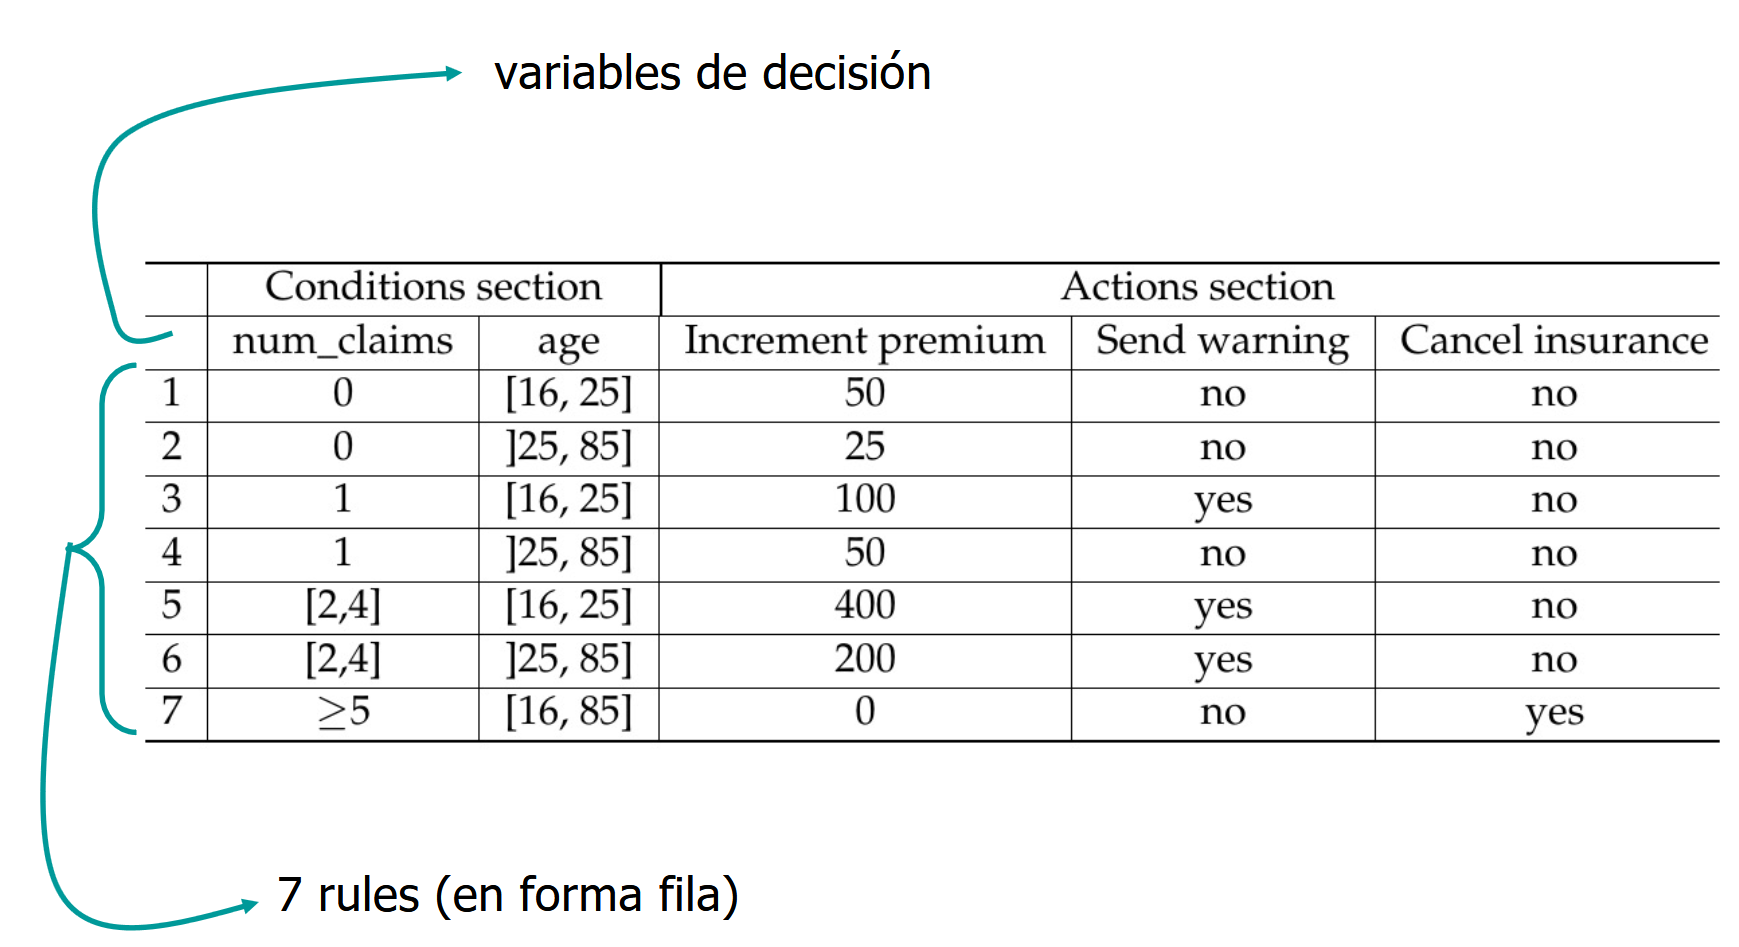
\includegraphics{images/05/tablaForma2.png}
   \caption{Forma columna y forma fila de tablas de decisión}
   \label{fig:05/tablaForma}
\end{figure}

\section{Valores Límites}
\begin{itemize}
	\item Intervalo: un subconjunto del espacio de los valores de entrada de
un programa.
	\item Punto límite de un intervalo (boundary) : aquel punto que según
sea incrementado o decrementado un valor epsilon infinitesimal
dará como resultado un valor perteneciente o no a dicho intervalo.
	\item Desigualdad del límite : una expresión algebraica con $>$, $<$, $\geq$, $\leq$
que define parte de los puntos que pertenecen a un intervalo o
dominio.
	\item Condiciones de igualdad : una expresión algebraica con $=$, $\neq$
\end{itemize}

\begin{figure}[htbp]
   \centering
   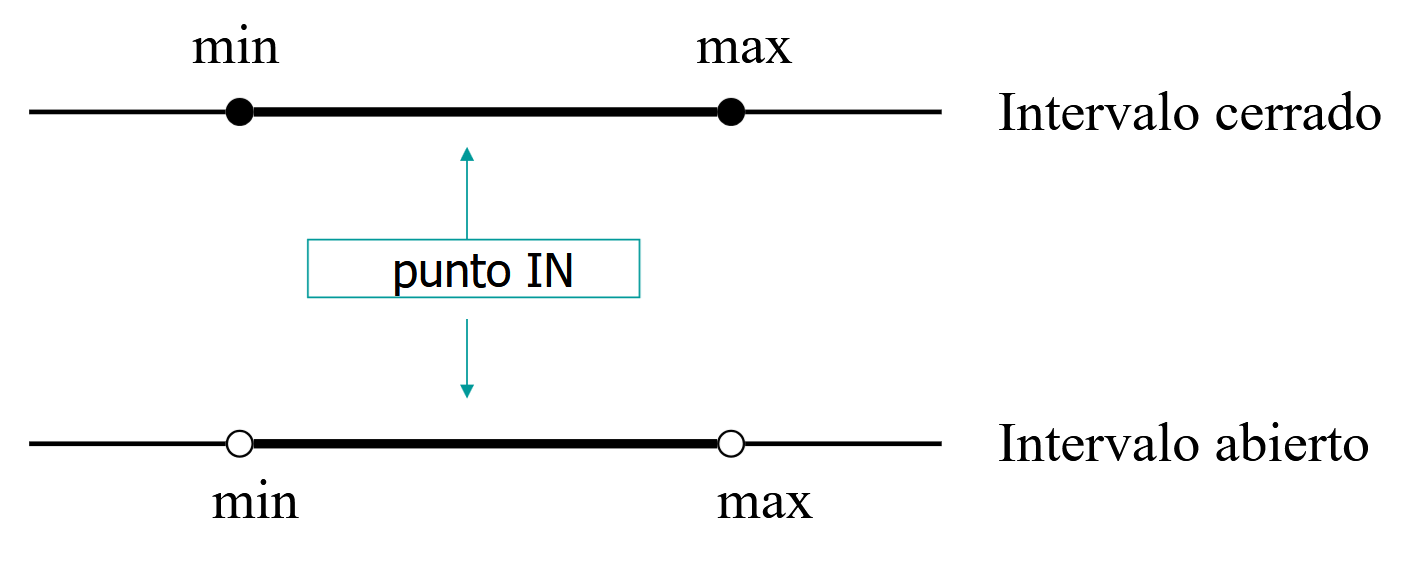
\includegraphics[width=0.45\columnwidth]{images/05/puntoIN.png}
   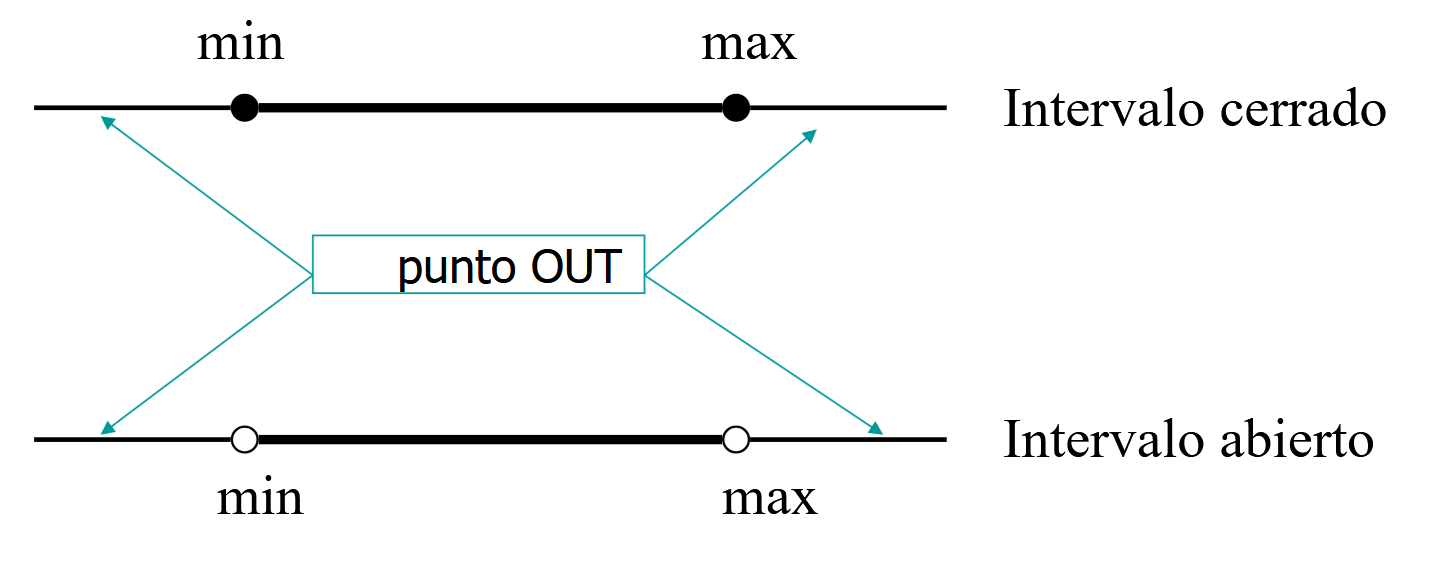
\includegraphics[width=0.45\columnwidth]{images/05/puntoOUT.png}
   \caption{puntoINOUT}
   \label{fig:05/puntoINOUT}
\end{figure}
\begin{figure}[htbp]
   \centering
   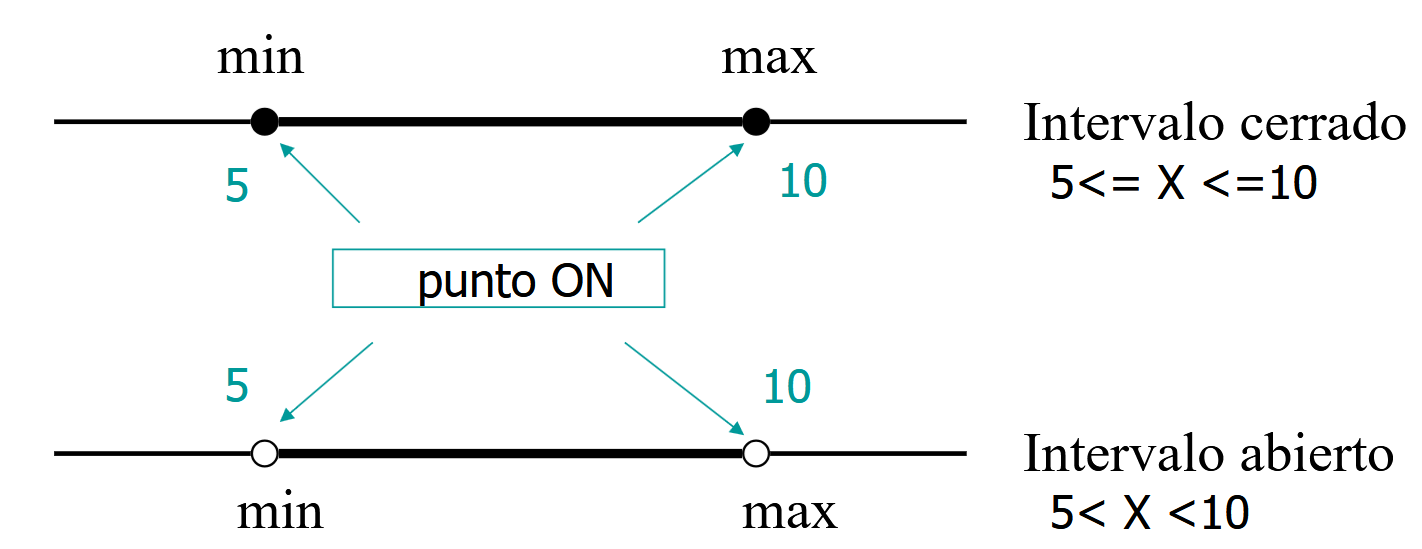
\includegraphics[width=0.45\columnwidth]{images/05/puntoON.png}
   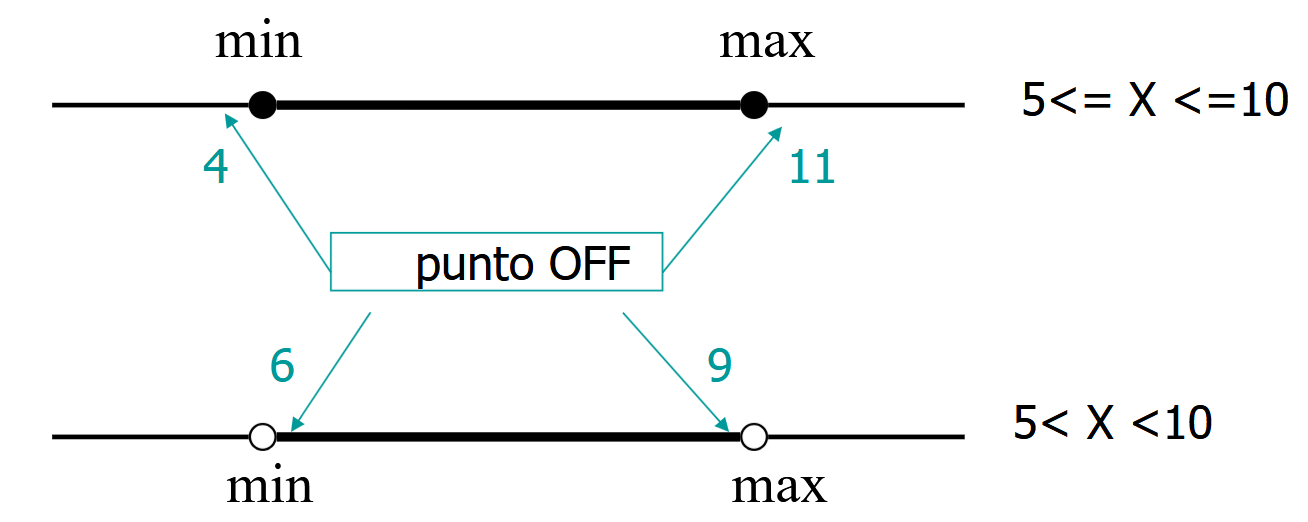
\includegraphics[width=0.45\columnwidth]{images/05/puntoOFF.png}
   \caption{puntoONOFF}
   \label{fig:05/puntoONOFF}
\end{figure}

\begin{itemize}
   \item \textsc{Punto IN} : un punto que pertenece al intervalo
   \item \textsc{Punto OUT} : un punto que no pertenece al intervalo
   \item \textsc{Punto ON} : un punto que pertenece al intervalo y es un límite
   \item \textsc{Punto OFF} : un valor cerca del punto límite de un intervalo
\end{itemize}

La estrategia para diseñar las pruebas de valores límites es 1 punto ON + 1 punto OFF para cada desigualdad de límite.
\note{Ejemplos:
\begin{itemize}
	\item 3 <= extras < 10
	      \begin{itemize}
		      \item Puntos ON: extras = 3; extras = 10
		      \item Puntos OFF: extras = 2; extras = 9
	      \end{itemize}
	\item 2000 < precio\_base <= 5000
	      \begin{itemize}
		      \item Puntos ON?
		      \item Puntos OFF?
	      \end{itemize}
\end{itemize}}


\chapter{Cyber-Physical Systems}

\section{Introducción}


\begin{definition}
   [CPS]
   A cyber-physical system is a system of collaborating computational
   elements controlling physical entities
\end{definition}
Cyber-Physical System (CPS) is a generic term for a variety of
control systems, such as SCADA (Supervisory Control and Data
Acquisition) systems, ICSs (Industrial Control Systems), BCSs
(Building Control Systems), and the global electrical smart grid

\begin{definition}
   [CPS - 2]
   A Cyber Physical System (CPS) is a network of interacting and
   collaborating computational elements controlling physical entities,
   including sensors, actuators, control processing units, and
   communication devices
\end{definition}

\begin{definition}
   [CPS - 3]
   CPS are systems used to monitor and control the physical world
\end{definition}

\begin{definition}
   [CPS - 4]
   CPS are IT systems that are integrated into physical world application
\end{definition}

\framedt{Events out of temperatures}{
   Consideremos un escenario en el que se mide la temperatura con un sensor.
   Para saber si la temperatura es alta o baja, se necesita un umbral, lo que se llama un \textbf{valor de referencia}.\\
   Esto permite de comparar la temperatura medida con el valor de referencia y tomar una decisión, como por ejemplo generar una alarma si la temperatura es demasiado alta.
}

\section{Componenetes de CPSs}

CPS tienen vulnerabilidades específicas, porque hay:
\begin{itemize}
	\item Issolation asumption
	\item Increased connectivity
	\item Heterogeneity
	\item Long life cycle of components
	\note{Hay softwares que todavía necesitan Windows XP}
\end{itemize}

\begin{figure}[htbp]
   \centering
   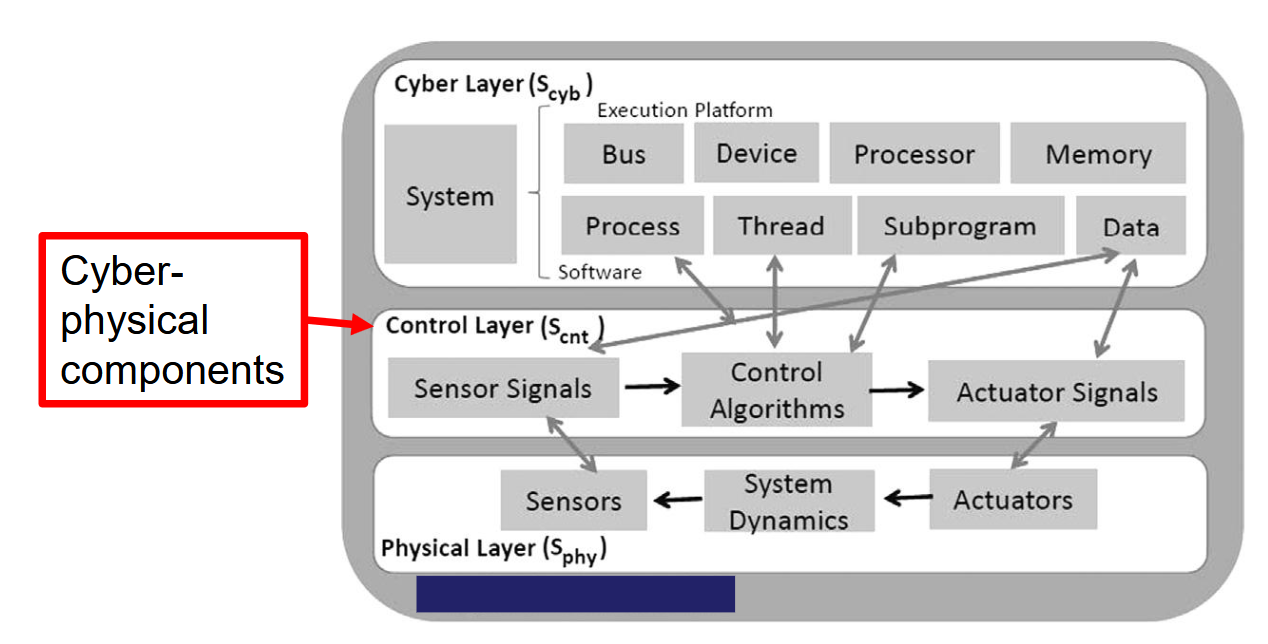
\includegraphics{images/06/CPScomponents.png}
   \caption{Cyberphysical Components}
   \label{fig:06/CPScomponents}
\end{figure}


\subsubsection{Industrial Control Systems}
Sometimes are called SCADA (Supervisory Control and Data Acquisition) systems or DCS (Distributed Control Systems).

El ejemplo más común de ICS son las redes de PLC, por wired o wireless. Tradicionalmente, los PLCs se comunican con un SCADA a través ambos de un protocolo OT (Operational Technologies) de comunicación propietario y de los protocolos IT standard.\\
Tradicionalmente, la isolación era la mejor defensa para estos sistemas.
Patching y updates son un problema, porque los sistemas no pueden ser apagados, y entonces no pueden ser parcheados.

SCADA systems se componen de 4 niveles:
\begin{enumerate}
	\item Sensors and actuators
	\item Distributed controllers, which include programmable logic
   controllers (PLCs), intelligent electronic devices (IEDs), and
   other forms of programmable automation controllers (PACs)
	\item Supervisory and control systems, which encompasses
   systems that store process data, and implements control
   schemes to manage the lower levels
	\item Human machine interfaces (HMIs), which enable the human
   operators to manage the physical process
\end{enumerate}

Diferencias entre ICS y sistemas IT:
\begin{itemize}
	\item Logic execution has a big impact on the physical environtment
	\item Edge devices are, at least, so relevant as hosts servers
	\item Computation resources of edge devices are usually very limited
	\item Safety is the most relevant design constrain
	\item Continuous availability and time-critically constrains
	\item Hard-Real time vs Soft-Real time vs Best-Effort systems
\end{itemize}

SCADA network components:
\begin{itemize}
	\item Servers and workstations that are used by operators to
interact with the field devices segment
	\item HMI software-based graphical user interface
	\item Monitoring of field devices
	\item Field devices data updating
	\item Historian systems
	\item Back up systems (similar to IT systems)
\end{itemize}

Field devices components:
\begin{itemize}
	\item Programmable Logic Controllers (PLCs)
	\item Remote Terminal Units (RTUs)
	\item Intelligent Electronic Devices (IEDs)
	\item IEDs are microprocessor based devices as sensors, motors (actuators),
brakes,lights, etc
	\item IEDs are controled by RTUs and PLCs by mean of field buses
protocols (as PROFIBUS DP)
	\item RTUs monitor IEDs and transmit data to PLCs using ModBUS RTU and
DNP3
	\item Sometimes, directed to the SCADA network using ModBUS TCP
	\item PLCs are control computers, with many types of I/O interfaces
\end{itemize}

Usual incidents in ICSs:
\begin{itemize}
	\item Blocked or delayed flow of information through ICS networks, which could
disrupt ICS operation
	\item Unauthorized changes to instructions, commands, or alarm thresholds, which
could damage, disable, or shut down equipment, create environmental
impacts, and/or endanger human life
	\item Inaccurate information sent to system operators, either to disguise
unauthorized changes, or to cause the operators to initiate inappropriate
actions, which could have various negative effects
	\item ICS software or configuration settings modified, or ICS software infected with
malware, which could have various negative effects
	\item Interference with the operation of equipment protection systems, which could
endanger costly and difficult-to-replace equipment
	\item Interference with the operation of safety systems, which could endanger
human life
\end{itemize}

\section{Vulnerabilidades}
\begin{enumerate}
	\item Vulnerabilities inherent in the CPS product, or platform
vulnerabilities
	\item Vulnerabilities because of poor network design or
configuration, or network equipment vulnerabilities
	\item Vulnerabilities caused during the installation, configuration,
and maintenance of the CPS, or management vulnerabilities
\end{enumerate}

\begin{figure}[htbp]
	\centering
	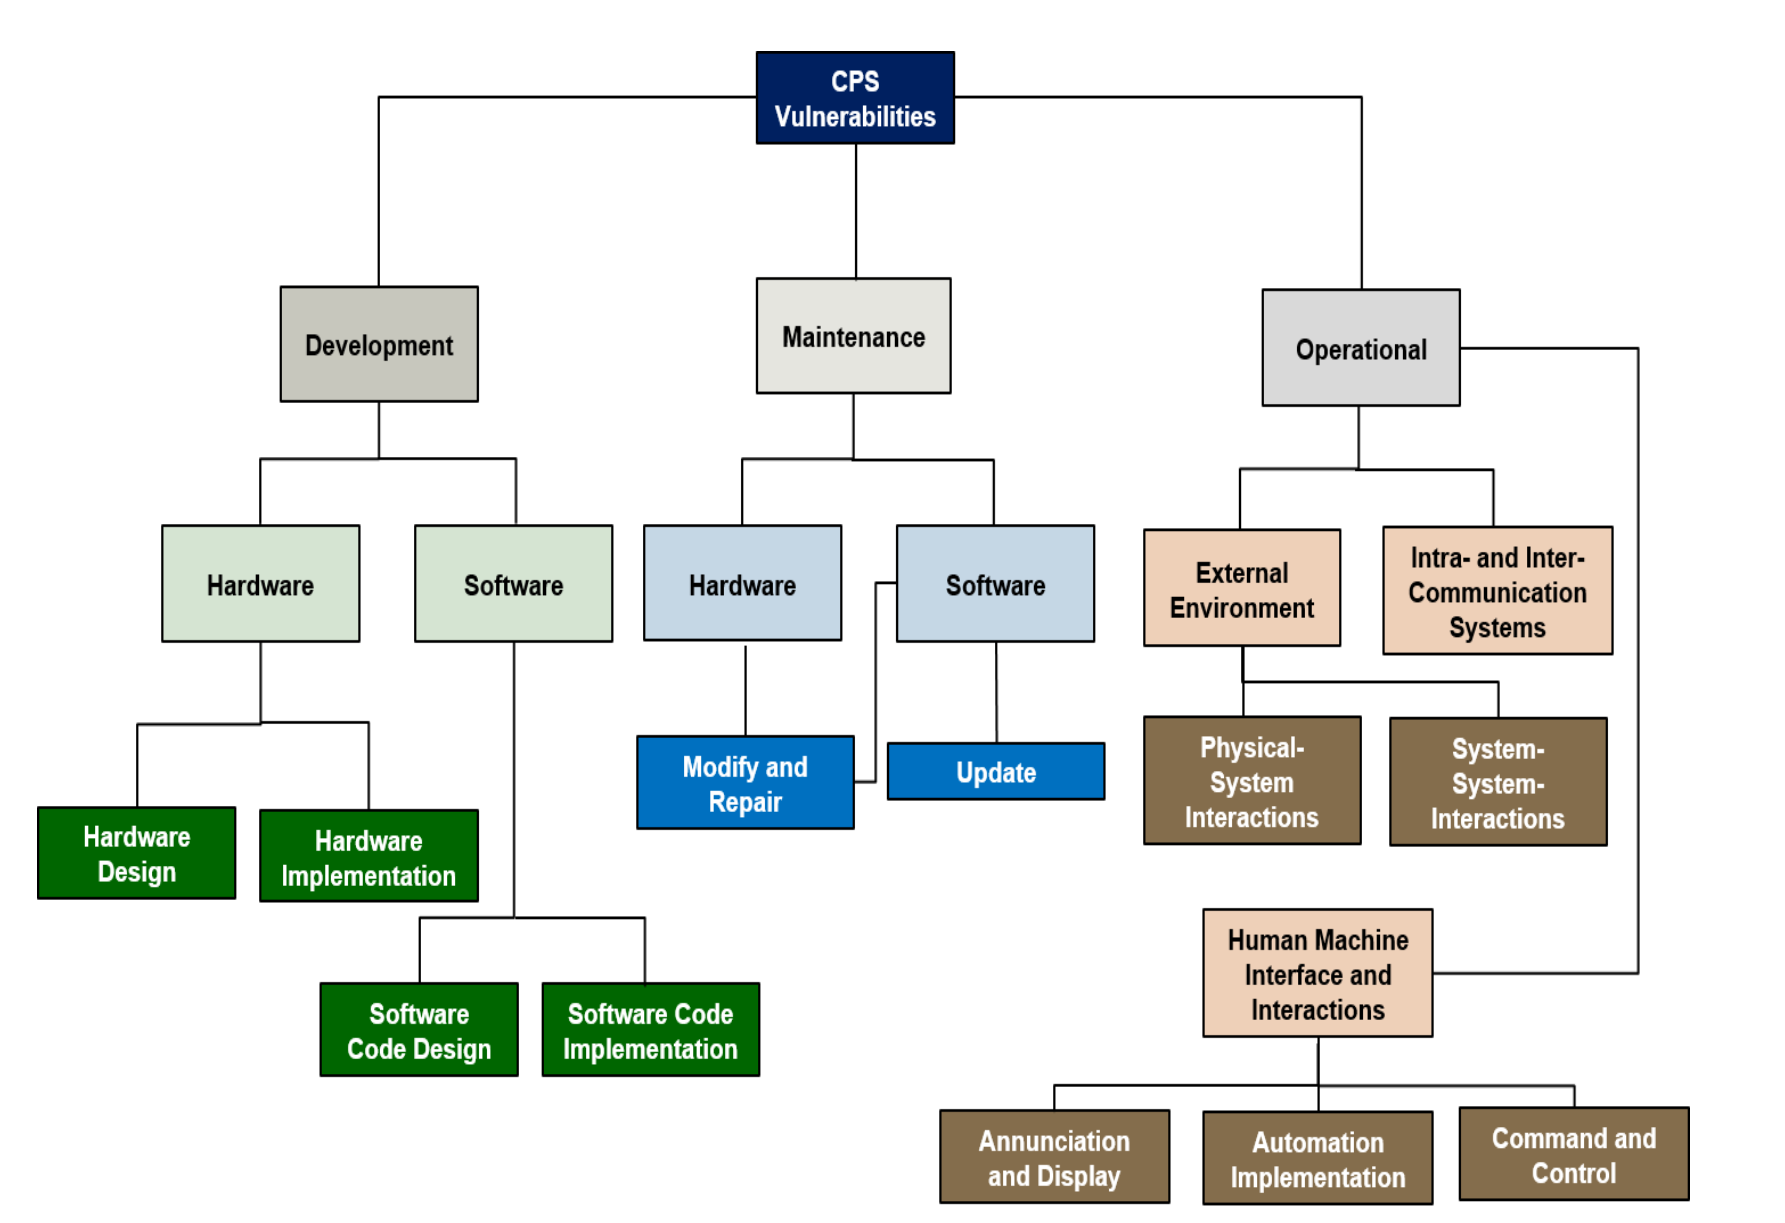
\includegraphics{images/07/cpsVulns.png}
	\caption{CPS Vulnerabilidades taxonomía}
	\label{fig:07/cpsVulns}
\end{figure}

A la izquierda de la figura \ref{fig:07/cpsVulns} hay una lista de vulnerabilidades son vulnerabilidades de plataforma, al centro hay vulnerabilidades de la gestión, y a la derecha vulnerabilidades operacionales.\\
Cómo hemos dicho antes, tipicamente es difícil actualizar el software para CPSs, esto es el motivo por el cual hay muchas vulnerabilidades relacionadas a la mantenimiento del software.

Las vulnerabilidades más comunes son:
\begin{itemize}
	\item Improper Input Validation / Validación incorrecta de las entradas
	\item Permissions, Privileges and Access Control / Permisos, privilegios y control de acceso
	\item Improper Authentication / Autenticación incorrecta
	\item Insufficient Verification of Data Authenticity / Verificación insuficiente de la autenticidad de los datos
	\item Poor Code Quality / Código de baja calidad
	\item Security Configuration and Maintenance / Configuración y mantenimiento de la seguridad
	\item Credentials Management / Gestión de credenciales
\end{itemize}

\subsection{Vulnerabilidades más comunes}
La más explotada vulnerabilidad en CPSs es \textbf{Buffer Overflow}, que es tipicamente permitida por la falta de validación de las entradas: los programadores suelen tener en cuenta lo que debería ocurrir y lo que podría ocurrir por error, pero no todas las posibilidades maliciosas.

Malas prácticas de código permiten a los atacantes suministrar datos inesperados y modificar así la ejecución del programa. Esta vulnerabilidad se llama \textbf{Lack of Bounds Checking}.


\textbf{Cross-Site scripting} vulnerabilidades pueden ser explotadas para muchos tipos de ataques, como el \textbf{Cross-Site Request Forgery} (CSRF), que permite a un atacante ejecutar comandos en el contexto de un usuario autenticado. En general, el Cross-Site Scripting permite \textbf{Code Injection}. 

\section{Vulnerabilities Assessment}
Para los CPS, los objetivos de seguridad están en orden inverso de prioridad, siendo la disponibilidad considerada la más importante, en lugar de la confidencialidad. El personal de la industria a menudo usa el término "seguridad" para referirse a la disponibilidad y fiabilidad del sistema.

Nada debe hacerse en una red CPS activa que pueda interferir o interrumpir las operaciones críticas del sistema. En el entorno CPS, los objetivos de seguridad del mundo IT son reemplazados por la salud y seguridad humana, la disponibilidad del sistema, y la puntualidad e integridad de los datos. Esta es la principal diferencia entre las evaluaciones de seguridad de CPS y de IT.

Esta diferencia también se aplica a las estrategias de mitigación. Ninguna solución de ciberseguridad puede implementarse en la red CPS si interfiere con la respuesta del sistema. El equipo de evaluación cibernética debe trabajar con el personal de la industria y los proveedores para realizar una evaluación efectiva sin comprometer la seguridad, disponibilidad o integridad del CPS.

CPS Vulnerabilities Assessment Execution Phases:
\begin{enumerate}
	\item \textbf{Reconnaissance} -
	The first part of a cyber security assessment is to identify a
target to attack.
	\item \textbf{Exploration} -
	Once a target has been identified, the assessment team attacks
the system
	\item \textbf{Exploit development} -
	Once a problem has been identified, the assessment team may
optionally develop an exploit for the vulnerability.
\item[] All these phases have specific aspects in CPS vulnerabilities assessment
\end{enumerate}

\subsection{Intrusion detection}

HIDS no se utilizan mucho en ICSs, porque ---tipicamente--- no se puede instalar software sobre CPS components.
Entonces, se utilizan \textbf{Network IDS} basados sobre \textbf{anomalias}.
La detección por firmas (signature-based) tiene buena precisión para IT sistemas, pero no lo es para ICSs, porque \dots // TODO

La detección por firmas (signature-based) tiene buena precisión para IT sistemas, pero no lo es para ICSs, porque tiene que depender de firmas conocidas y actualizadas, mientras que los protocolos y comportamientos en entornos ICS son muy específicos y a menudo propietarios.

% \subsection{Lateral Movements}

\textbf{Lateral Movements} son muy comunes en ICSs, porque los atacantes pueden moverse lateralmente a través de la red para obtener acceso a otros sistemas, y entonces, \textbf{honeypots} son una defensa muy eficaz para detectar y monitorear estos movimientos. Los honeypots simulan componentes legítimos del sistema, atrayendo a los atacantes y permitiendo analizar sus técnicas sin comprometer los sistemas reales.

La segmentación de la red, junto con controles de acceso estrictos entre zonas, también es fundamental para limitar la capacidad de los atacantes de moverse lateralmente una vez que han comprometido un punto de entrada inicial en la red ICS.

\subsection{Exploits mitigación}

En general es muy difícil mitigar los exploits en CPSs, porque no se pueden aplicar parches a los sistemas.

% // TODO




\end{document}
